GreenWUP, presentato in \cite{greenWup}, è un protocollo \textit{cross-layer} (Routing + MAC) usato nelle \textit{Green Wireless Sensor Network} che fa uso di tecnologie come \textit{energy-harvesting}, \textit{wake-up radio} e \textit{semantic-addressing} al fine di migliorare il consumo energetico della rete e in generale le sue prestazioni.  \\

GreenWUP è un protocollo \textit{converge-casting} basato sugli \textit{hop-count}. Infatti, è molto importante che ogni nodo della rete sia a conoscenza della propria distanza dal sink in termini di hop.\\
Questo valore, nel caso di GreenWUP, è calcolato automaticamente, infatti, conoscendo il raggio di azione delle 2 antenne (principale e di wake-up) e conoscendo la posizione esatta dei nodi è possibile stabilire per ogni nodo la sua distanza dal sink.\\

Tuttavia per questo progetto si è deciso di calcolare questo valore mediante un prima fase iniziale chiamata \textit{Interest Dissemination} usando il protocollo \textit{FloodWUP}.\\

Altra caratteristica molto importante per il corretto funzionamento di GreenWUP è che ogni nodo ha associato, all'interno di una stessa rete, due indirizzi di wake-up:
\begin{enumerate}
    \item \textbf{w\textsubscript{ID}}, un indirizzo statico che identifica univocamente il nodo all'interno della rete 
    \item \textbf{w\textsubscript{LE}}, un indirizzo dinamico con semantica che identifica lo stato in cui un nodo si trova in un determinato istante
\end{enumerate}
L'indirizzo \textbf{w\textsubscript{ID}} è un semplice intero progressivo che identifica i vari nodi assegnando un ID da \textit{0} a \textit{n} se si hanno \textit{n} nodi.\\
L'indirizzo \textbf{w\textsubscript{LE}}, invece, è ricalcolato periodicamente in quanto deve rappresentare lo stato attuale del nodo. In particolare è formato da due sequenze \(w_{L}w_{E}\) dove w\textsubscript{L} è la codifica del valore di hop-count del nodo e w\textsubscript{E} è l'energia residua del nodo. Nello specifico i vari livelli di energia sono discretizzati in \textit{k} classi\footnote{Ogni classe comprende un range di valori di energia, per cui un nodo con energia residua \textit{x} appartiene alla classe \textit{k} sse \(energiaResidua(nodo)\in range(\texitf{k})\)} per cui w\textsubscript{E} è la classe energetica a cui, attualmente, il nodo appartiene.\\

\'E possibile dividere in fasi l'invio di un  pacchetto DATA, inviato ovviamente da un nodo \textit{sender}\footnote{Nodo che detiene un pacchetto DATA da inoltrare verso il \textit{sink}} verso il \textit{next-hop}\footnote{Nodo vicino al \textit{sender} che riceve il pacchetto DATA da questo}:
\begin{itemize}
    \item \textit{Relay Selection}: in questa prima fase il sender prova ad instaurare una comunicazione con i receiver\footnote{Nodi vicini del sink che potrebbero essere scelti come \texitit{next-hop} }. Infatti si utilizza l'indirizzo di wake-up \textbf{w\textsubscript{LE}}. Questa procedura si considera conclusa nel momento in cui il nodo sender ha scelto, tra i propri vicini, chi sarà il next-hop.
    \item \textit{Send DATA}: in questa fase il nodo sender sollecita, mediante l'indirizzo di wake-up \textbf{w\textsubscript{ID}}, il next-hop e procede poi con l'invio del pacchetto DATA.
    \item \textit{Send ACK}: in questa fase finale il nodo next-hop, dopo aver correttamente ricevuto il pacchetto DATA, invia un ACK al nodo sender in modo da confermare la ricezione.
\end{itemize}
Un'osservazione importante è che se il next-hop si trova a distanza 1 dal sink, la fase di \textit{Relay Selection} viene saltata. Infatti il nodo sink è sempre in ascolto per cui si procede direttamente con l'invio del pacchetto DATA e con il successivo pacchetto ACK.\\\\

\begin{figure}[h!]
  \begin{subfigure}[t]{.8\linewidth}
    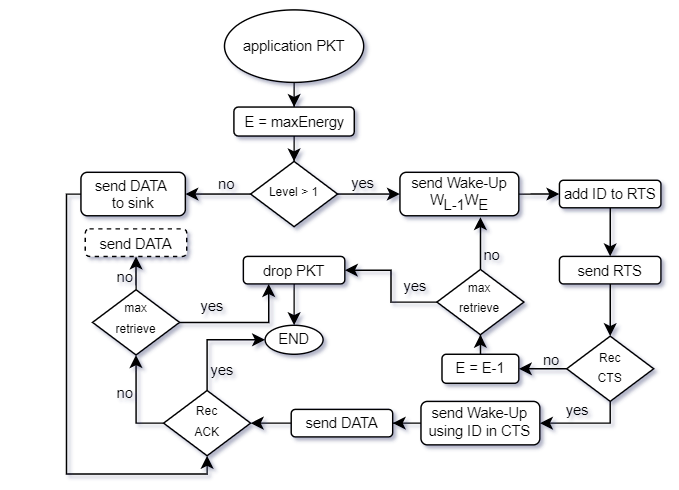
\includegraphics[width=1.15\linewidth]{Contents/Images/schemes/greenWupBase/GreenWup_base_sender.png}
  \end{subfigure}
  \caption{Logica funzionamento nodo \texitit{sender}}
  \label{fig:logicaSender}
\end{figure}

La \textbf{Figura \ref{fig:logicaSender}} sopra riportata mostra il comportamento di un nodo sender una volta che questo ha un pacchetto DATA da gestire.\\

Bisogna precisare che il nodo sink si occuperà della sola ricezione di pacchetti DATA per cui mai per nessun motivo il sink eseguirà questa procedura.\\
Come mostrato dalla \textbf{Figura \ref{fig:logicaSender}}, all'inzio la classe di energia considerata è la massima. A questo punto se il nodo è un vicino del sink, per cui \(level=1\), si salta come già detto la fase di Relay Selection e si invia direttamente il dato al sink. Altrimenti vengono sollecitati i vicini in base alla loro distanza dal sink e alla loro classe energetica. Si noti che il sender memorizza all'interno del pacchetto RTS il proprio indirizzo univoco in modo da essere ricontattato poi per ricevere il CTS.\\
Qualora non dovesse ricevere nessun pacchetto CTS, il sender riproverebbe con una classe energetica più bassa un numero massimo di volte, per poi eliminare il pacchetto e terminare la procedura.\\
Se, invece, il nodo sender dovesse ricevere il pacchetto CTS, solleciterebbe il vicino usando l'indirizzo univoco contenuto all'interno del CTS per poi mandaere il pacchetto DATA e successivamente si metterebbe in attesa dell'acknowledge. Se il nodo riceve l'ACK allora conclude la procedura, altrimenti ritenta l'invio del pacchetto per un massimo numero di volte per poi eliminarlo e terminare la procedura.\\\\

\begin{figure}[h!]
  \begin{subfigure}[t]{.8\linewidth}
    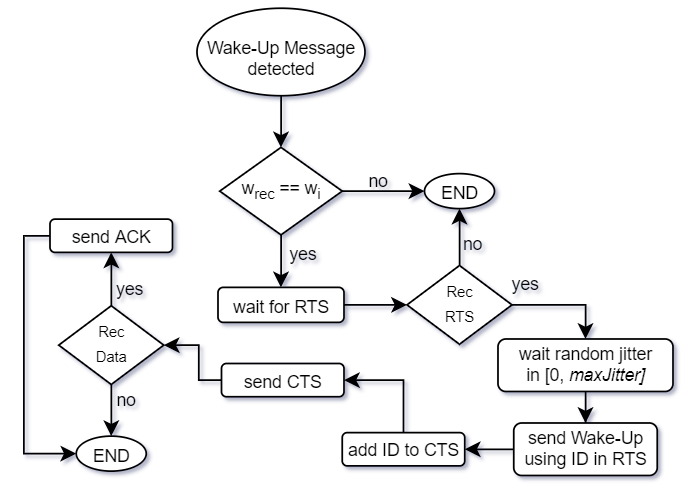
\includegraphics[width=1.1\linewidth]{Contents/Images/schemes/greenWupBase/GreenWup_base_receiver.png}
  \end{subfigure}
  \caption{Logica funzionamento nodo \texitit{receiver}}
  \label{fig:logicaReceiver}
\end{figure}

La \textbf{Figura \ref{fig:logicaReceiver}} sopra riportata mostra il comportamento di un nodo receiver una volta che questo viene sollecitato da un vicino tramite un messaggio di wake-up.\\
La prima cosa che fa un nodo receiver è controllare che la sequenza di wake-up con cui è stato sollecitato corrisponda a \(w_{i}\) dove \(w_{i} \in (w_{ID}, w_{LE})\). Se così non dovesse essere allora ignora il pacchetto e la procedura finisce, altrimenti si mette in attesa di un pacchetto RTS da parte del sender. Una volta ricevuto si aspetta un tempo calcolato randomicamente per poi sollecitare il nodo sender usando le informazioni contenute nel pacchetto RTS. Una volta sollecitato il nodo sender, il receiver procede con la creazione del pacchetto CTS con le proprie informazioni e, una volta creato, lo invia al sender.\\
A questo punto il receiver non può far altro che mettersi in attesa del pacchetto DATA. Ovviamente solo il receiver scelto come \textit{next-hop} riceverà il pacchetto DATA, per poi proseguire con l'invio dell'acknowledge. Per tutti gli altri scatterà un \textit{timeout} che terminerà la procedura.